\documentclass[11pt,a4paper]{article}

% Packages
\usepackage[utf8]{inputenc}
\usepackage[T1]{fontenc}
\usepackage{geometry}
\geometry{margin=1in}
\usepackage{graphicx}
\usepackage{amsmath,amssymb}
\usepackage{booktabs}
\usepackage{hyperref}
\usepackage{caption}
\usepackage{subcaption}
\usepackage{tikz}
\usetikzlibrary{shapes.geometric, arrows.meta, positioning, fit, backgrounds, calc}
\usepackage{pgfplots}
\pgfplotsset{compat=1.18}
\usepackage{xcolor}
\usepackage{enumitem}
\usepackage{float}

% Color definitions
\definecolor{deepblue}{RGB}{31,78,121}
\definecolor{deepred}{RGB}{192,57,43}
\definecolor{deepgreen}{RGB}{39,174,96}
\definecolor{lightblue}{RGB}{52,152,219}
\definecolor{lightyellow}{RGB}{255,245,200}
\definecolor{terran}{RGB}{0,100,200}
\definecolor{protoss}{RGB}{200,160,0}
\definecolor{zerg}{RGB}{160,32,240}
\definecolor{gmcolor}{RGB}{255,200,200}

\title{\textbf{Survey Report: Grandmaster Level in StarCraft~II\\Using Multi-Agent Reinforcement Learning}\\[0.5em]
\large A Comprehensive Summary of the AlphaStar System\\[0.3em]
\normalsize ECE 752 --- Advanced Computer Architecture}
\author{Summary of Vinyals, O.\ et al.\ (Nature, 2019)}
\date{}

\begin{document}
\maketitle

\begin{abstract}
This report provides a comprehensive survey of the DeepMind AlphaStar system, as presented in ``Grandmaster Level in StarCraft~II Using Multi-Agent Reinforcement Learning'' (Vinyals et al., \textit{Nature} 575, 350--354, 2019). AlphaStar is the first artificial intelligence agent to reach Grandmaster level in the full game of StarCraft~II, placing above 99.8\% of officially ranked human players across all three playable races. The system combines deep neural network architectures, imitation learning from human replays, multi-agent reinforcement learning via a novel league training procedure, and operates under human-like constraints including camera restrictions and action-rate limits. This report details the game environment, the agent architecture, the training pipeline, the multi-agent league framework, empirical evaluation results, ablation studies, and broader implications for AI research.
\end{abstract}

\tableofcontents
\newpage

%=============================================================================
\section{Introduction}
%=============================================================================

Many real-world applications require artificial agents to compete and coordinate with other agents in complex, partially observable environments. StarCraft~II, developed by Blizzard Entertainment, has long served as a grand challenge for artificial intelligence research. It is one of the most popular and difficult professional esports, featuring:

\begin{itemize}[nosep]
    \item A \textbf{combinatorial action space} with approximately $10^{26}$ possible choices at each step.
    \item \textbf{Imperfect information} due to fog of war and a camera-based interface.
    \item \textbf{Long time horizons} spanning tens of thousands of time-steps per game ($\sim$10 minutes of real-time play).
    \item \textbf{Non-transitive strategy dynamics} (rock--paper--scissors cycles among strategies).
    \item \textbf{Three distinct races} (Terran, Protoss, Zerg) with fundamentally different mechanics.
\end{itemize}

Prior to AlphaStar, the strongest AI agents for StarCraft either simplified important aspects of the game, used superhuman capabilities (e.g., viewing the entire map simultaneously or issuing thousands of actions per minute), or relied on hand-crafted sub-systems. No previous agent came close to matching the overall skill of top human players in the unmodified game.

AlphaStar addresses these challenges using \emph{general-purpose} machine learning methods---combining neural network architectures, imitation learning, reinforcement learning, and multi-agent training---that are in principle applicable to any complex domain. The resulting agent was evaluated on Blizzard's official Battle.net matchmaking system and achieved Grandmaster-level ratings for all three races, placing above 99.8\% of ranked human players on the European server.

%=============================================================================
\section{The StarCraft~II Domain}
%=============================================================================

\subsection{Game Overview}

StarCraft~II is a real-time strategy (RTS) game in which players balance high-level economic decisions with individual control of hundreds of units. The most common competitive setting is 1v1, where each player selects one of three races:

\begin{itemize}[nosep]
    \item \textbf{Terran}: Human-like faction with flexible, mechanized units.
    \item \textbf{Protoss}: Technologically advanced race with powerful but expensive units.
    \item \textbf{Zerg}: Biological swarm race emphasizing rapid production and adaptation.
\end{itemize}

Players begin with a small base and a few worker units, gather resources, construct buildings, research technologies, scout opponents, and build armies. A player is defeated when all their buildings are destroyed.

\subsection{Challenges for AI}

Figure~\ref{fig:challenges} illustrates the key challenges that make StarCraft~II a formidable AI benchmark.

\begin{figure}[H]
\centering
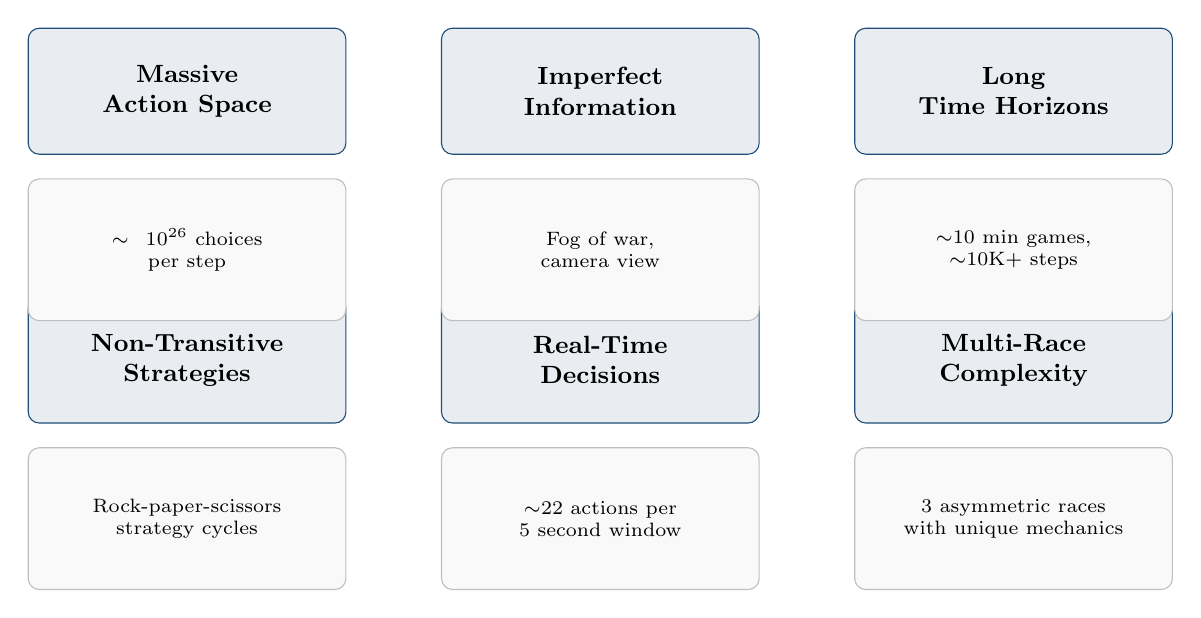
\begin{tikzpicture}[
    node distance=0.6cm and 1.2cm,
    challenge/.style={rectangle, rounded corners, draw=deepblue, fill=deepblue!10, text width=3.8cm, minimum height=1.6cm, align=center, font=\small\bfseries},
    desc/.style={rectangle, rounded corners, draw=gray!50, fill=gray!5, text width=3.8cm, minimum height=1.8cm, align=center, font=\scriptsize},
]
    % Challenge boxes
    \node[challenge] (c1) {Massive\\Action Space};
    \node[challenge, right=of c1] (c2) {Imperfect\\Information};
    \node[challenge, right=of c2] (c3) {Long\\Time Horizons};

    \node[challenge, below=1.8cm of c1] (c4) {Non-Transitive\\Strategies};
    \node[challenge, below=1.8cm of c2] (c5) {Real-Time\\Decisions};
    \node[challenge, below=1.8cm of c3] (c6) {Multi-Race\\Complexity};

    % Description boxes
    \node[desc, below=0.3cm of c1] {$\sim10^{26}$ choices\\per step};
    \node[desc, below=0.3cm of c2] {Fog of war,\\camera view};
    \node[desc, below=0.3cm of c3] {$\sim$10 min games,\\$\sim$10K+ steps};
    \node[desc, below=0.3cm of c4] {Rock-paper-scissors\\strategy cycles};
    \node[desc, below=0.3cm of c5] {$\sim$22 actions per\\5 second window};
    \node[desc, below=0.3cm of c6] {3 asymmetric races\\with unique mechanics};
\end{tikzpicture}
\caption{Key challenges of StarCraft~II as an AI benchmark. The combination of these factors makes it substantially harder than previous game-playing benchmarks such as chess, Go, or Atari.}
\label{fig:challenges}
\end{figure}

\subsection{Observation and Action Spaces}

At each time step $t$, the agent receives an observation $o_t$ that includes:
\begin{itemize}[nosep]
    \item A list of all observable units and their attributes (up to 512 entities).
    \item A 128$\times$128 spatial map with height, visibility, creep, entity ownership, and pathability layers.
    \item Player data: race, upgrades, resource counts, supply, and army statistics.
    \item Game statistics: camera position and in-game time.
\end{itemize}

Each action $a_t$ is highly structured, consisting of:
\begin{itemize}[nosep]
    \item \textbf{Action type}: what to do (move, attack, build, etc.).
    \item \textbf{Selected units}: which units execute the action.
    \item \textbf{Target}: an entity or map location (discretized to 256$\times$256).
    \item \textbf{Queued}: whether to queue or execute immediately.
    \item \textbf{Delay}: how many time-steps to wait before the next observation.
\end{itemize}

This representation results in approximately $10^{26}$ possible choices at each step, making direct enumeration infeasible.

%=============================================================================
\section{AlphaStar Architecture}
%=============================================================================

Central to AlphaStar is a policy $\pi_\theta(a_t \mid s_t, z) = \mathbb{P}[a_t \mid s_t, z]$, implemented as a deep neural network with parameters $\theta$. The network receives all observations from the start of the game as inputs and selects actions as outputs. The policy is also conditioned on a statistic $z$ that summarizes a strategy sampled from human data (e.g., a build order). Figure~\ref{fig:architecture} provides a high-level overview of the architecture.

\begin{figure}[H]
\centering
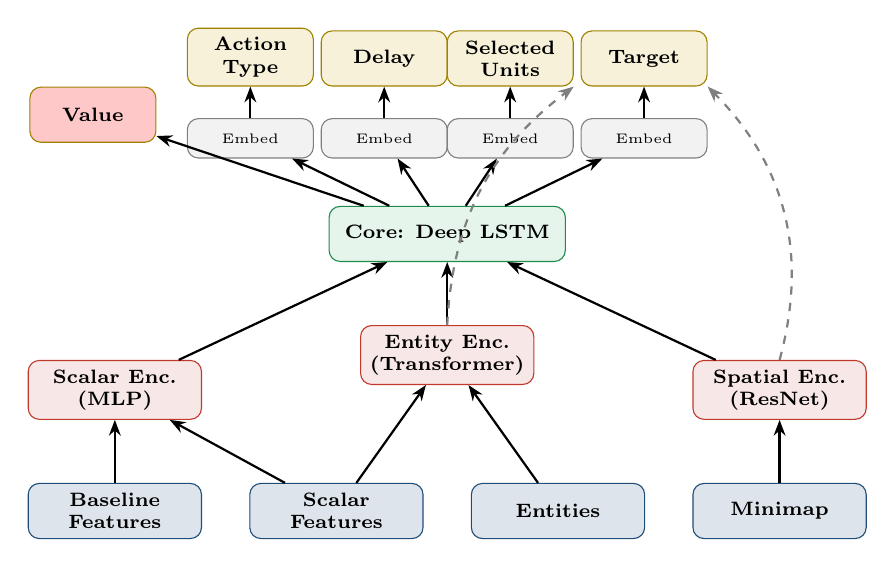
\begin{tikzpicture}[
    node distance=0.5cm and 0.4cm,
    input/.style={rectangle, rounded corners, draw=deepblue, fill=deepblue!15, minimum width=2.2cm, minimum height=0.7cm, align=center, font=\scriptsize\bfseries},
    encoder/.style={rectangle, rounded corners, draw=deepred, fill=deepred!12, minimum width=2.2cm, minimum height=0.7cm, align=center, font=\scriptsize\bfseries},
    core/.style={rectangle, rounded corners, draw=deepgreen!80!black, fill=deepgreen!12, minimum width=3cm, minimum height=0.7cm, align=center, font=\scriptsize\bfseries},
    output/.style={rectangle, rounded corners, draw=protoss!80!black, fill=protoss!15, minimum width=1.6cm, minimum height=0.7cm, align=center, font=\scriptsize\bfseries},
    embed/.style={rectangle, rounded corners, draw=gray, fill=gray!10, minimum width=1.6cm, minimum height=0.5cm, align=center, font=\tiny},
    arrow/.style={-{Stealth[length=2mm]}, thick},
    darrow/.style={-{Stealth[length=2mm]}, thick, dashed, gray},
]
    % Input layer
    \node[input] (baseline) {Baseline\\Features};
    \node[input, right=0.6cm of baseline] (scalar) {Scalar\\Features};
    \node[input, right=0.6cm of scalar] (entities) {Entities};
    \node[input, right=0.6cm of entities] (minimap) {Minimap};

    % Encoder layer
    \node[encoder, above=0.8cm of baseline] (scenc) {Scalar Enc.\\(MLP)};
    \node[encoder, above=0.8cm of scalar] (entenc) at ($(scalar)!0.5!(entities) + (0, 0.8)$) {Entity Enc.\\(Transformer)};
    \node[encoder, above=0.8cm of minimap] (spatenc) {Spatial Enc.\\(ResNet)};

    % Core
    \node[core, above=0.8cm of entenc] (core) {Core: Deep LSTM};

    % Embedding layer
    \node[embed, above=0.6cm of core, xshift=-2.5cm] (emb1) {Embed};
    \node[embed, above=0.6cm of core, xshift=-0.8cm] (emb2) {Embed};
    \node[embed, above=0.6cm of core, xshift=0.8cm] (emb3) {Embed};
    \node[embed, above=0.6cm of core, xshift=2.5cm] (emb4) {Embed};

    % Output heads
    \node[output, above=0.4cm of emb1] (act) {Action\\Type};
    \node[output, above=0.4cm of emb2] (delay) {Delay};
    \node[output, above=0.4cm of emb3] (sel) {Selected\\Units};
    \node[output, above=0.4cm of emb4] (tgt) {Target};

    % Value head
    \node[output, above=0.8cm of core, xshift=-4.5cm, fill=gmcolor] (val) {Value};

    % Arrows: inputs to encoders
    \draw[arrow] (baseline) -- (scenc);
    \draw[arrow] (scalar) -- (scenc);
    \draw[arrow] (scalar) -- (entenc);
    \draw[arrow] (entities) -- (entenc);
    \draw[arrow] (minimap) -- (spatenc);

    % Arrows: encoders to core
    \draw[arrow] (scenc) -- (core);
    \draw[arrow] (entenc) -- (core);
    \draw[arrow] (spatenc) -- (core);

    % Arrows: core to embeddings
    \draw[arrow] (core) -- (emb1);
    \draw[arrow] (core) -- (emb2);
    \draw[arrow] (core) -- (emb3);
    \draw[arrow] (core) -- (emb4);

    % Arrows: embeddings to outputs
    \draw[arrow] (emb1) -- (act);
    \draw[arrow] (emb2) -- (delay);
    \draw[arrow] (emb3) -- (sel);
    \draw[arrow] (emb4) -- (tgt);

    % Value arrow
    \draw[arrow] (core) -- (val);

    % Skip connections (dashed)
    \draw[darrow] (entenc.north) to[bend left=25] (sel.south east);
    \draw[darrow] (spatenc.north) to[bend right=30] (tgt.south east);

\end{tikzpicture}
\caption{High-level overview of the AlphaStar neural network architecture. Observations are processed by specialized encoders (scalar MLP, entity Transformer, spatial ResNet), integrated through a deep LSTM core, and decoded into structured action outputs via auto-regressive heads. Skip connections (dashed) allow direct information flow from entity encoders to the pointer network (selected units) and from spatial encoders to the target head. The model has 139 million parameters total, though only 55 million are needed during inference.}
\label{fig:architecture}
\end{figure}

\subsection{Input Encoders}

\begin{itemize}[nosep]
    \item \textbf{Scalar Encoder (MLP)}: Processes non-spatial features such as resource counts, supply, race information, and the strategy statistic $z$.
    \item \textbf{Entity Encoder (Transformer)}: Processes the variable-length list of up to 512 game entities using self-attention mechanisms, with scatter connections to integrate spatial and non-spatial information.
    \item \textbf{Spatial Encoder (ResNet)}: Processes the 128$\times$128 minimap layers using a residual convolutional network.
\end{itemize}

\subsection{Core: Deep LSTM}

The encoded representations are combined and fed into a deep Long Short-Term Memory (LSTM) network. The LSTM maintains memory across time steps, which is critical for handling partial observability---the agent must remember information about unseen areas of the map and track opponent activities over time.

\subsection{Output Heads (Auto-Regressive Decoding)}

The action space is decomposed into structured sub-actions, each predicted by a specialized output head conditioned on previous sub-action selections:

\begin{enumerate}[nosep]
    \item \textbf{Action Type} (Residual MLP): Selects what action to perform.
    \item \textbf{Delay} (MLP): Determines when to observe next.
    \item \textbf{Queued} (MLP): Whether to queue the action.
    \item \textbf{Selected Units} (Pointer Network): Which units to command.
    \item \textbf{Target Unit} (Attention): Which entity to target.
    \item \textbf{Target Point} (Deconvolutional ResNet): Where on the map to act.
\end{enumerate}

This auto-regressive decomposition via the chain rule reduces the intractable $10^{26}$-dimensional action space into a sequence of manageable categorical decisions.

\subsection{Value Network}

A separate value function $V_\theta(s_t, z)$ estimates the expected outcome of the game from the current state. During training, the value function uses \emph{both} the player's and the opponent's observations to reduce variance, though opponent information is not used during evaluation.

%=============================================================================
\section{Training Pipeline}
%=============================================================================

AlphaStar's training proceeds in two main phases: supervised learning from human replays, followed by reinforcement learning within a multi-agent league. Figure~\ref{fig:training_pipeline} illustrates this pipeline.

\begin{figure}[H]
\centering
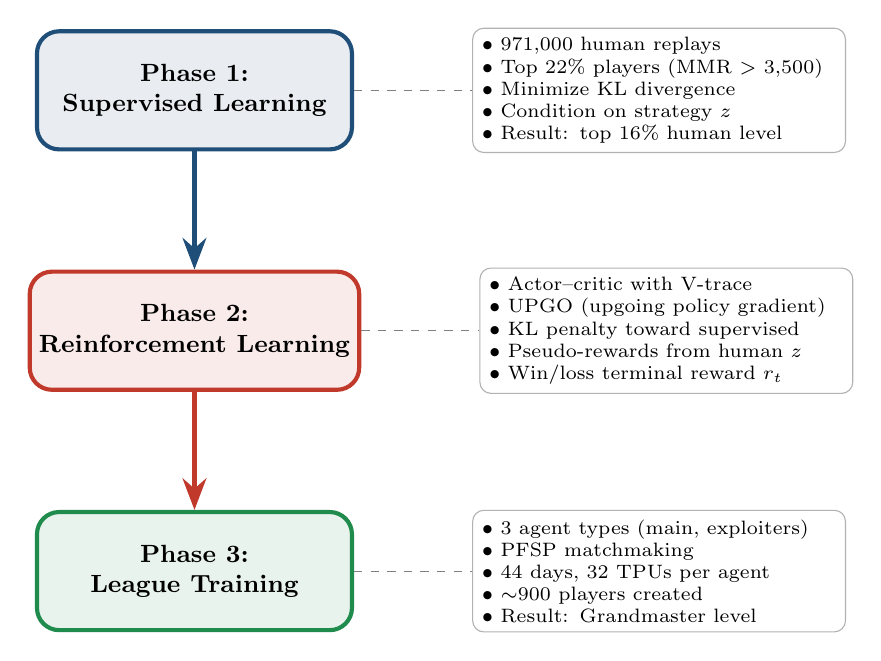
\begin{tikzpicture}[
    node distance=0.8cm and 0.8cm,
    phase/.style={rectangle, rounded corners=8pt, draw=#1, fill=#1!10, minimum width=4cm, minimum height=1.5cm, align=center, font=\small\bfseries, line width=1.5pt},
    detail/.style={rectangle, rounded corners, draw=gray!60, fill=white, text width=4.5cm, align=left, font=\scriptsize},
    bigarrow/.style={-{Stealth[length=4mm, width=3mm]}, line width=2pt, #1},
]
    % Phase 1
    \node[phase=deepblue] (sl) {Phase 1:\\Supervised Learning};
    \node[detail, right=1.5cm of sl] (sld) {
        $\bullet$ 971,000 human replays\\
        $\bullet$ Top 22\% players (MMR $>$ 3,500)\\
        $\bullet$ Minimize KL divergence\\
        $\bullet$ Condition on strategy $z$\\
        $\bullet$ Result: top 16\% human level
    };

    % Phase 2
    \node[phase=deepred, below=1.5cm of sl] (rl) {Phase 2:\\Reinforcement Learning};
    \node[detail, right=1.5cm of rl] (rld) {
        $\bullet$ Actor--critic with V-trace\\
        $\bullet$ UPGO (upgoing policy gradient)\\
        $\bullet$ KL penalty toward supervised\\
        $\bullet$ Pseudo-rewards from human $z$\\
        $\bullet$ Win/loss terminal reward $r_t$
    };

    % Phase 3
    \node[phase=deepgreen!80!black, below=1.5cm of rl] (league) {Phase 3:\\League Training};
    \node[detail, right=1.5cm of league] (leagued) {
        $\bullet$ 3 agent types (main, exploiters)\\
        $\bullet$ PFSP matchmaking\\
        $\bullet$ 44 days, 32 TPUs per agent\\
        $\bullet$ $\sim$900 players created\\
        $\bullet$ Result: Grandmaster level
    };

    % Arrows
    \draw[bigarrow=deepblue] (sl) -- (rl);
    \draw[bigarrow=deepred] (rl) -- (league);

    % Detail connections
    \draw[gray, dashed] (sl) -- (sld);
    \draw[gray, dashed] (rl) -- (rld);
    \draw[gray, dashed] (league) -- (leagued);

\end{tikzpicture}
\caption{The three-phase training pipeline of AlphaStar. Supervised learning bootstraps the policy from human replays, reinforcement learning refines it through self-play, and league training produces a diverse, robust population of agents that avoid strategic cycling.}
\label{fig:training_pipeline}
\end{figure}

\subsection{Phase 1: Supervised Learning}

AlphaStar is initially trained on a publicly available dataset of 971,000 replays from StarCraft~II, filtered to games by players with MMR scores above 3,500 (top 22\%). One policy is trained per race with the same architecture used during reinforcement learning. Key details:

\begin{itemize}[nosep]
    \item For each replay, a statistic $z$ is extracted encoding the player's build order (first 20 constructed buildings and units) and cumulative statistics (units, buildings, effects, and upgrades present during the game).
    \item The policy is trained to predict each human action $a_t$ conditioned on either $s_t$ alone or on $(s_t, z)$, with $z$ set to zero 10\% of the time.
    \item The loss is the KL divergence between the model's output distribution and the human actions, optimized with Adam and $L_2$ regularization.
    \item Fine-tuning on replays with MMR above 6,200 (16,000 games) further improves win rate from 87\% to 96\% against built-in Protoss vs.\ Protoss elite bots.
\end{itemize}

The supervised agents achieved fine-tuned MMR ratings of 3,947 (Terran), 3,607 (Protoss), and 3,544 (Zerg), placing them in approximately the top 16\% of human players.

\subsection{Phase 2: Reinforcement Learning}

Reinforcement learning refines the supervised policy to maximize win rate. The terminal reward is $r_T \in \{-1, 0, +1\}$ (loss, draw, win) with no discount. Key algorithmic components:

\begin{itemize}[nosep]
    \item \textbf{Actor--Critic Framework}: Based on the advantage actor--critic algorithm, with updates applied asynchronously on replayed experience (off-policy learning).
    \item \textbf{V-trace}: Clipped importance sampling to correct for the mismatch between the behavior policy and the current policy in the large action space.
    \item \textbf{TD($\lambda$)}: Temporal difference learning for value function estimation.
    \item \textbf{UPGO (Upgoing Policy Gradient)}: A novel algorithm that updates the policy only from partial trajectories with better-than-expected returns, bootstrapping when the behavior policy takes a worse-than-average action. This helps the agent learn from successful sub-trajectories.
    \item \textbf{KL Regularization}: A penalty is applied whenever the agent's action probabilities differ from the supervised policy, maintaining exploration of human-like strategies throughout training.
    \item \textbf{Pseudo-Rewards}: Agents receive additional rewards for following the strategy statistic $z$ (measured by edit distance between sampled and executed build orders, and Hamming distance on cumulative statistics), encouraging diverse strategic exploration.
\end{itemize}

The overall loss is a weighted sum of the win-loss reward, the V-trace policy and value losses, UPGO, pseudo-reward losses, the KL divergence with the supervised policy, and entropy regularization.

\subsection{Phase 3: League Training (Multi-Agent RL)}

League training is a novel multi-agent reinforcement learning framework designed to address the non-transitive strategy dynamics in StarCraft~II (where strategy A beats B, B beats C, but C beats A). Figure~\ref{fig:league} illustrates the league structure.

\begin{figure}[H]
\centering
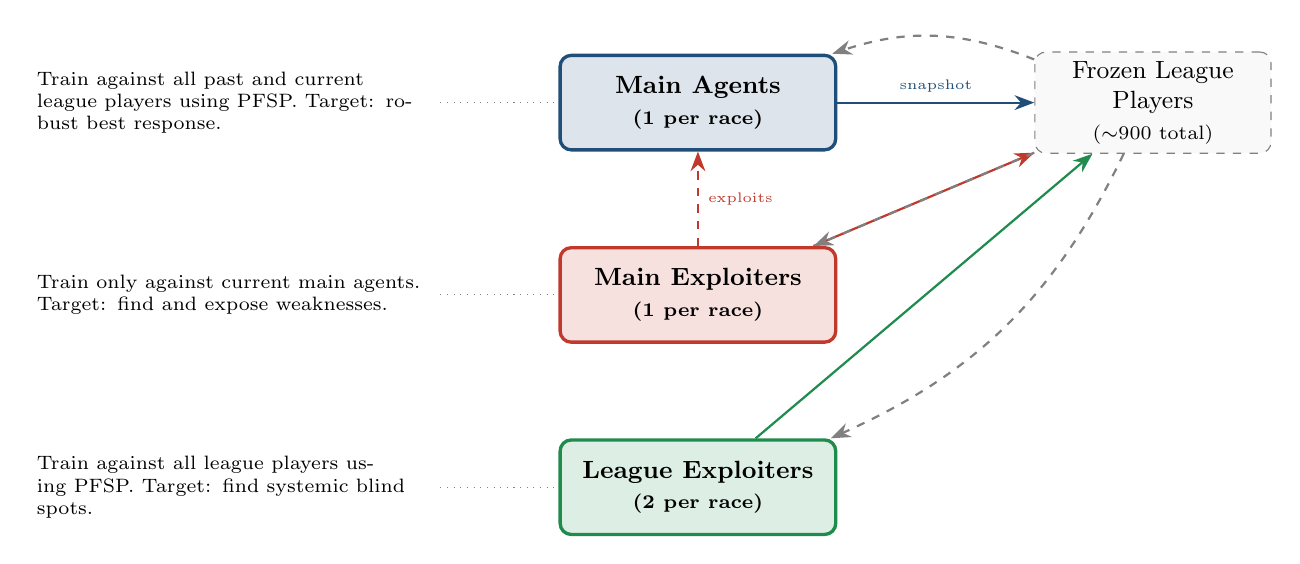
\begin{tikzpicture}[
    node distance=0.5cm and 1.5cm,
    agent/.style={rectangle, rounded corners, draw=#1, fill=#1!15, minimum width=3.5cm, minimum height=1.2cm, align=center, font=\small\bfseries, line width=1.2pt},
    desc/.style={text width=5cm, align=left, font=\scriptsize},
    arrow/.style={-{Stealth[length=2.5mm]}, thick, #1},
]
    % Main agents
    \node[agent=deepblue] (main) {Main Agents\\{\scriptsize (1 per race)}};

    % Main exploiters
    \node[agent=deepred, below=1.2cm of main] (mexploit) {Main Exploiters\\{\scriptsize (1 per race)}};

    % League exploiters
    \node[agent=deepgreen!80!black, below=1.2cm of mexploit] (lexploit) {League Exploiters\\{\scriptsize (2 per race)}};

    % Frozen players (league)
    \node[draw=gray, dashed, fill=gray!5, rounded corners, minimum width=3cm, minimum height=1cm, right=2.5cm of main, align=center, font=\small] (league) {Frozen League\\Players\\{\scriptsize ($\sim$900 total)}};

    % Descriptions
    \node[desc, left=1.5cm of main] (md) {Train against all past and current league players using PFSP. Target: robust best response.};
    \node[desc, left=1.5cm of mexploit] (med) {Train only against current main agents. Target: find and expose weaknesses.};
    \node[desc, left=1.5cm of lexploit] (led) {Train against all league players using PFSP. Target: find systemic blind spots.};

    % Arrows to league
    \draw[arrow=deepblue] (main) -- node[above, font=\tiny]{snapshot} (league);
    \draw[arrow=deepred] (mexploit) -- (league);
    \draw[arrow=deepgreen!80!black] (lexploit) -- (league);

    % Arrows from league
    \draw[arrow=gray, dashed] (league) to[bend right=20] (main);
    \draw[arrow=gray, dashed] (league) to[bend right=0] (mexploit);
    \draw[arrow=gray, dashed] (league) to[bend left=20] (lexploit);

    % Arrows between agents
    \draw[arrow=deepred, dashed] (mexploit) -- node[right, font=\tiny]{exploits} (main);

    % Description connections
    \draw[gray, dotted] (md) -- (main);
    \draw[gray, dotted] (med) -- (mexploit);
    \draw[gray, dotted] (led) -- (lexploit);

\end{tikzpicture}
\caption{Structure of the AlphaStar league. Three types of agents interact: main agents seek robust performance against the full league, main exploiters specifically target weaknesses in main agents, and league exploiters search for systemic blind spots across the entire population. All agents periodically snapshot frozen copies into the league, growing the pool of diverse opponents.}
\label{fig:league}
\end{figure}

\subsubsection{Prioritized Fictitious Self-Play (PFSP)}

Standard Fictitious Self-Play (FSP) computes a best response against a uniform mixture of all previous policies, which converges to a Nash equilibrium in two-player zero-sum games. AlphaStar extends this with \textbf{Prioritized FSP (PFSP)}, which adapts the opponent mixture proportionally to the win rate of each opponent against the agent:

\begin{equation}
    f_{\text{hard}}(x) = (1-x)^p, \quad p \in \mathbb{R}_+
\end{equation}

where $x$ is the agent's current win rate against the opponent. This focuses training on the hardest opponents---those the agent currently struggles against---rather than wasting games against already-defeated opponents. This is critical in StarCraft because the pursuit of maximum \emph{average} win rate leads to easily exploitable policies in a game with highly non-transitive dynamics.

\subsubsection{Agent Types}

The league consists of three agent types with different roles:

\begin{enumerate}[nosep]
    \item \textbf{Main Agents}: Use PFSP (35\% self-play, 50\% PFSP, 15\% forgotten-player PFSP) against all players. These agents are never reset and form the final deployed policy.
    \item \textbf{Main Exploiters}: Train only against current main agents to identify potential weaknesses. They are periodically reset to supervised parameters, making main agents more robust.
    \item \textbf{League Exploiters}: Use PFSP against the entire league to find global blind spots. They too are periodically reset, helping discover specialist strategies that are not necessarily robust themselves.
\end{enumerate}

During 44 days of league training using 12 separate actor--learner setups (each with 32 TPUs), approximately 900 distinct players were created in the league.

%=============================================================================
\section{Human-Like Interface Constraints}
%=============================================================================

A critical design decision in AlphaStar is to impose constraints that approximate human physical limitations, ensuring fair comparison. Figure~\ref{fig:constraints} summarizes these constraints.

\begin{figure}[H]
\centering
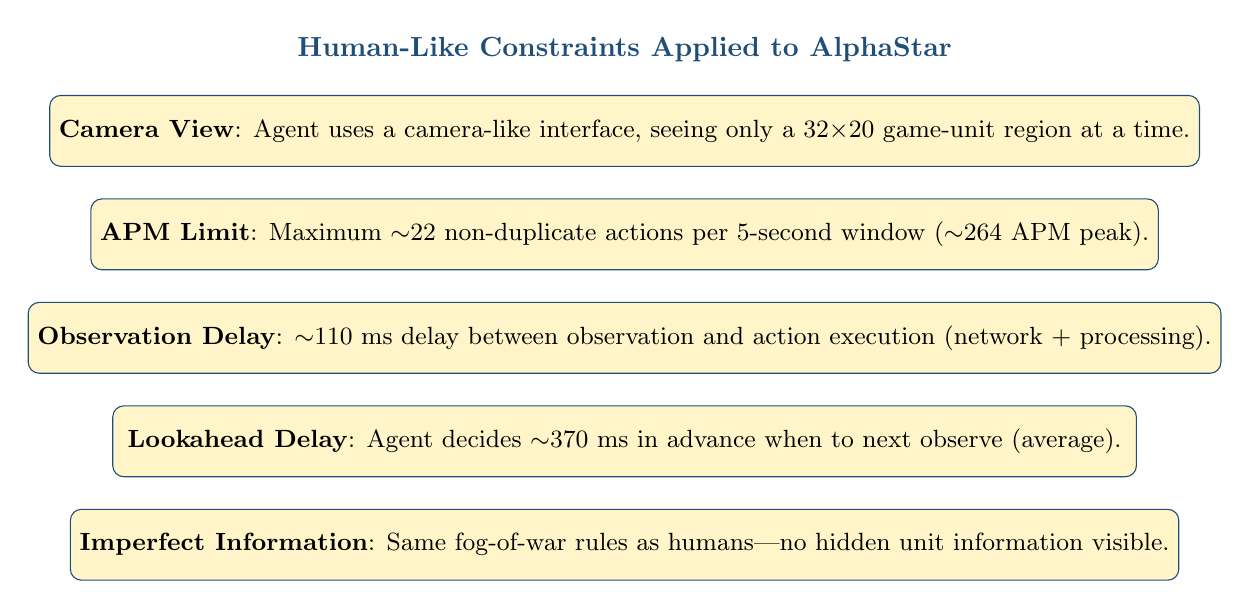
\begin{tikzpicture}[
    node distance=0.4cm,
    constraint/.style={rectangle, rounded corners, draw=deepblue, fill=lightyellow, minimum width=13cm, minimum height=0.9cm, align=left, font=\small},
]
    \node[constraint] (c1) {\textbf{Camera View}: Agent uses a camera-like interface, seeing only a 32$\times$20 game-unit region at a time.};
    \node[constraint, below=of c1] (c2) {\textbf{APM Limit}: Maximum $\sim$22 non-duplicate actions per 5-second window ($\sim$264 APM peak).};
    \node[constraint, below=of c2] (c3) {\textbf{Observation Delay}: $\sim$110 ms delay between observation and action execution (network + processing).};
    \node[constraint, below=of c3] (c4) {\textbf{Lookahead Delay}: Agent decides $\sim$370 ms in advance when to next observe (average).};
    \node[constraint, below=of c4] (c5) {\textbf{Imperfect Information}: Same fog-of-war rules as humans---no hidden unit information visible.};

    \node[above=0.3cm of c1, font=\bfseries\color{deepblue}] {Human-Like Constraints Applied to AlphaStar};
\end{tikzpicture}
\caption{Summary of the constraints imposed on AlphaStar to ensure a fair comparison with human players. These constraints were developed in consultation with professional StarCraft~II players and Blizzard employees.}
\label{fig:constraints}
\end{figure}

Ablation studies showed that these constraints significantly affect performance:
\begin{itemize}[nosep]
    \item Removing the camera interface increased win rate from 87\% to 94\% against the elite bot, demonstrating that camera management is a substantial challenge.
    \item Reducing APM substantially reduced performance, and unexpectedly, \emph{increasing} APM beyond the limit also reduced performance---because the agent spent more effort on micro-tactics rather than diverse strategic play.
\end{itemize}

%=============================================================================
\section{Empirical Results}
%=============================================================================

\subsection{Battle.net Evaluation}

AlphaStar was evaluated at three training snapshots on Blizzard's official Battle.net matchmaking system under blind conditions (anonymous account, no opponent identity information):

\begin{table}[H]
\centering
\caption{AlphaStar MMR ratings and human population percentiles on Battle.net. Grandmaster (GM) threshold is approximately 6,200 MMR on the European server.}
\label{tab:results}
\begin{tabular}{@{}lccccc@{}}
\toprule
\textbf{Agent} & \textbf{Training} & \textbf{Protoss} & \textbf{Terran} & \textbf{Zerg} & \textbf{Percentile} \\
\midrule
AlphaStar Supervised & SL only & 3,607 & 3,947 & 3,544 & $\sim$84\% \\
AlphaStar Mid & SL + 27d RL & 5,991 & 6,048 & 5,755 & $\sim$99.5\% \\
AlphaStar Final & SL + 44d RL & \textbf{6,275} & \textbf{6,048} & \textbf{5,835} & $>\textbf{99.8\%}$ \\
\midrule
Grandmaster Threshold & --- & \multicolumn{3}{c}{$\sim$6,200} & 99.8\% \\
\bottomrule
\end{tabular}
\end{table}

AlphaStar Final achieved Grandmaster level for all three races, with its highest rating of 6,275 MMR for Protoss. This places it above 99.8\% of approximately 90,000 ranked players on the European server.

\subsection{Performance Progression}

Figure~\ref{fig:mmr_progression} shows how AlphaStar's performance improved over the course of training.

\begin{figure}[H]
\centering
\begin{tikzpicture}
\begin{axis}[
    width=12cm, height=7cm,
    xlabel={Training Days},
    ylabel={MMR Rating},
    xmin=0, xmax=45,
    ymin=3000, ymax=6800,
    legend pos=south east,
    grid=major,
    grid style={gray!20},
    legend style={font=\small},
    fill between/on layer={axis background},
]
    % GM threshold
    \addplot[dashed, thick, gmcolor!80!red, domain=0:45] {6200};
    \addlegendentry{GM Threshold ($\sim$6200)}

    % Protoss
    \addplot[thick, protoss, mark=*, mark size=1.5pt] coordinates {
        (0,3607) (5,4200) (10,4800) (15,5300) (20,5700) (25,5900) (27,5991) (30,6050) (35,6150) (40,6230) (44,6275)
    };
    \addlegendentry{Protoss}

    % Terran
    \addplot[thick, terran, mark=square*, mark size=1.5pt] coordinates {
        (0,3947) (5,4400) (10,4900) (15,5350) (20,5650) (25,5850) (27,6048) (30,6030) (35,6040) (40,6045) (44,6048)
    };
    \addlegendentry{Terran}

    % Zerg
    \addplot[thick, zerg, mark=triangle*, mark size=2pt] coordinates {
        (0,3544) (5,4000) (10,4600) (15,5000) (20,5400) (25,5600) (27,5755) (30,5770) (35,5800) (40,5820) (44,5835)
    };
    \addlegendentry{Zerg}

    % Annotation
    \node[anchor=west, font=\scriptsize, text=gray] at (axis cs:1,6400) {Grandmaster};
\end{axis}
\end{tikzpicture}
\caption{Approximate MMR progression of AlphaStar over 44 days of league training for each race. Day 0 corresponds to the supervised learning baseline. All three races surpass or approach the Grandmaster threshold ($\sim$6,200 MMR) by the end of training.}
\label{fig:mmr_progression}
\end{figure}

\subsection{Actions Per Minute (APM) Comparison}

AlphaStar's effective APM was constrained to be comparable to or lower than human professionals. As reported by StarCraft~II:

\begin{table}[H]
\centering
\caption{Effective actions per minute (EPM) statistics for AlphaStar Final (blue) and human opponents (red) on Battle.net.}
\label{tab:apm}
\begin{tabular}{@{}lccc@{}}
\toprule
& \textbf{Average EPM} & \textbf{99.9th \%ile EPM} & \textbf{Max EPM} \\
\midrule
\textit{Terran --- AlphaStar} & 183 & 487 & 571 \\
\textit{Terran --- Human} & 200 & 554 & 755 \\
\midrule
\textit{Protoss --- AlphaStar} & 187 & 509 & 587 \\
\textit{Protoss --- Human} & 205 & 537 & 621 \\
\midrule
\textit{Zerg --- AlphaStar} & 211 & 655 & 823 \\
\textit{Zerg --- Human} & 259 & 823 & 1192 \\
\bottomrule
\end{tabular}
\end{table}

Notably, AlphaStar's peak APM statistics are \emph{substantially lower} than those of human opponents, confirming that the agent does not rely on superhuman speed.

%=============================================================================
\section{Ablation Studies}
%=============================================================================

Extensive ablation experiments were conducted on a simplified setup (one map, Protoss vs.\ Protoss, $10^{10}$ training steps, with Elo ratings estimated against 11,000 games with the built-in StarCraft~II bots). Figure~\ref{fig:ablations} summarizes the key findings.

\begin{figure}[H]
\centering
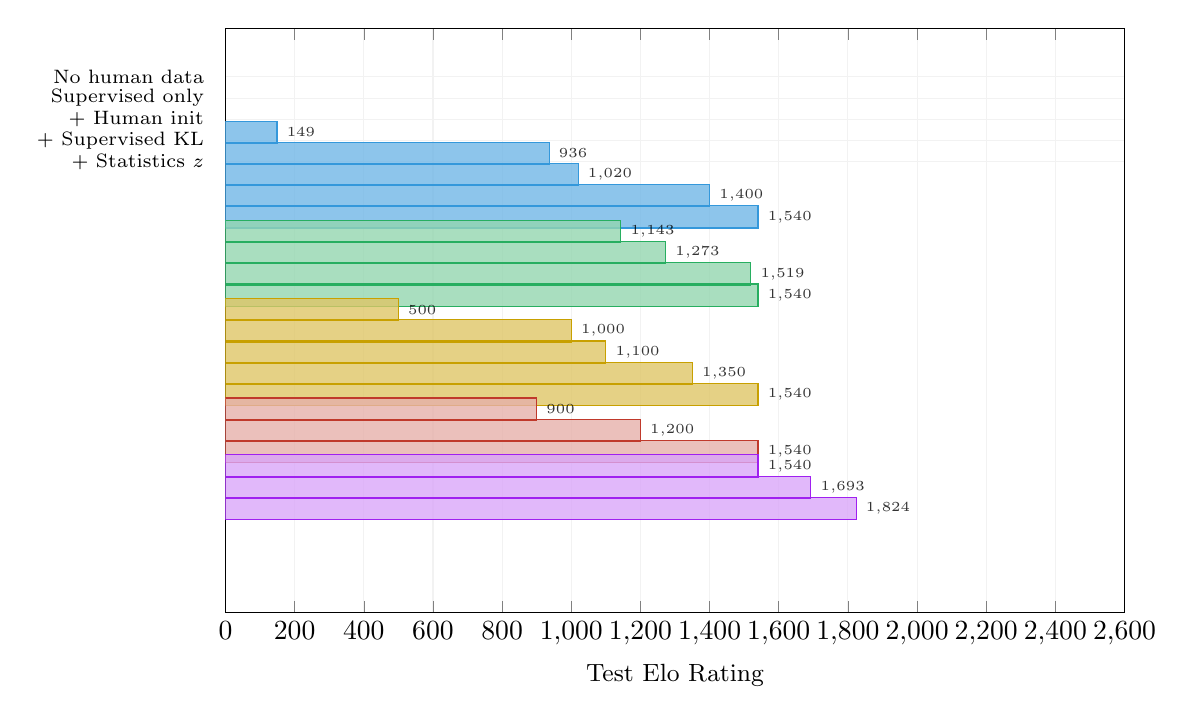
\begin{tikzpicture}
\begin{axis}[
    width=13cm, height=9cm,
    xbar,
    xlabel={Test Elo Rating},
    xlabel style={font=\small},
    xmin=0, xmax=2600,
    ytick=data,
    yticklabels={
        {No human data},
        {Supervised only},
        {+ Human init},
        {+ Supervised KL},
        {+ Statistics $z$},
        {},
        {FSP},
        {PFSP},
        {SP (self-play)},
        {pFSP + SP},
        {},
        {Baseline (no attn.)},
        {+ Action delays},
        {+ Pointer network},
        {+ Transformer},
        {+ Scatter connections},
        {},
        {V-Trace only},
        {+ TD($\lambda$)},
        {+ UPGO},
        {},
        {Main agents only},
        {+ Main exploiters},
        {+ League exploiters}
    },
    y dir=reverse,
    bar width=8pt,
    nodes near coords,
    nodes near coords style={font=\tiny, anchor=west},
    every axis plot/.append style={fill opacity=0.8},
    grid=major,
    grid style={gray!10},
    ytick style={draw=none},
    yticklabel style={font=\scriptsize, anchor=east},
]

    % Human data usage
    \addplot[fill=lightblue!70, draw=lightblue] coordinates {
        (149,1) (936,2) (1020,3) (1400,4) (1540,5)
    };

    % Multi-agent learning
    \addplot[fill=deepgreen!50, draw=deepgreen] coordinates {
        (1143,7) (1273,8) (1519,9) (1540,10)
    };

    % Architecture
    \addplot[fill=protoss!60, draw=protoss] coordinates {
        (500,12) (1000,13) (1100,14) (1350,15) (1540,16)
    };

    % Off-policy learning
    \addplot[fill=deepred!40, draw=deepred] coordinates {
        (900,18) (1200,19) (1540,20)
    };

    % League composition
    \addplot[fill=zerg!40, draw=zerg] coordinates {
        (1540,22) (1693,23) (1824,24)
    };

\end{axis}
\end{tikzpicture}
\caption{Summary of ablation study results (Test Elo). Each bar shows the performance contribution of a component. Human data, PFSP-based multi-agent learning, Transformer-based entity encoding with scatter connections, UPGO, and exploiter agents all provide significant improvements.}
\label{fig:ablations}
\end{figure}

\subsection{Key Ablation Findings}

\begin{enumerate}[nosep]
    \item \textbf{Human Data is Critical}: Removing all human data collapses performance to Elo 149. Even the supervised-only agent (Elo 936) benefits enormously from human initialization (1,020), KL regularization (1,400), and strategy conditioning $z$ (1,540).

    \item \textbf{Multi-Agent Learning}: PFSP + self-play (Elo 1,540) substantially outperforms pure self-play (1,519) and especially pure FSP (1,143). Adding exploiters raises league Elo from 1,540 (main agents only) to 1,824 (full league with all exploiters), an 18\% improvement.

    \item \textbf{Architecture}: The Transformer-based entity encoder, pointer network for unit selection, and scatter connections each contribute significantly. The baseline architecture without these components achieves only Elo $\sim$500.

    \item \textbf{Off-Policy Learning}: V-trace alone provides reasonable off-policy correction, but adding TD($\lambda$) and UPGO together yield the best combined performance.

    \item \textbf{Value Function}: Using opponent information as input to the value function (during training only) improves average win rate from 25\% to 82\%, a dramatic reduction in value estimation variance.

    \item \textbf{Camera Interface}: Using the non-camera interface yields a 94\% win rate vs.\ the elite bot, compared to 87\% with the camera---confirming that camera management is a meaningful component of skill.

    \item \textbf{APM Limits}: Reducing APM reduces performance as expected, but \emph{increasing} APM also reduces performance, as the agent spends more effort on micro-tactics rather than strategic diversity.
\end{enumerate}

%=============================================================================
\section{Training Infrastructure}
%=============================================================================

The scale of computation required to train AlphaStar is substantial. Figure~\ref{fig:infrastructure} illustrates the distributed training infrastructure.

\begin{figure}[H]
\centering
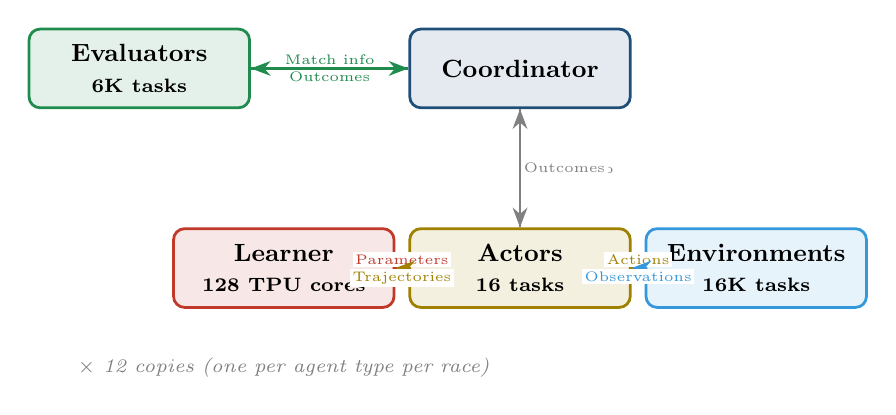
\begin{tikzpicture}[
    node distance=0.6cm and 1cm,
    component/.style={rectangle, rounded corners, draw=#1, fill=#1!12, minimum width=2.8cm, minimum height=1cm, align=center, font=\small\bfseries, line width=1pt},
    flow/.style={-{Stealth[length=2.5mm]}, thick, #1},
    label/.style={font=\tiny, midway, fill=white, inner sep=1pt},
]
    % Coordinator
    \node[component=deepblue] (coord) {Coordinator};

    % Evaluators
    \node[component=deepgreen!80!black, left=2cm of coord] (eval) {Evaluators\\{\scriptsize 6K tasks}};

    % Agent group
    \node[component=deepred, below=1.5cm of coord, xshift=-3cm] (learner) {Learner\\{\scriptsize 128 TPU cores}};
    \node[component=protoss!80!black, below=1.5cm of coord] (actors) {Actors\\{\scriptsize 16 tasks}};
    \node[component=lightblue, below=1.5cm of coord, xshift=3cm] (envs) {Environments\\{\scriptsize 16K tasks}};

    % Arrows
    \draw[flow=deepgreen!80!black] (eval) -- node[label, above]{Match info} (coord);
    \draw[flow=deepgreen!80!black] (coord) -- node[label, below]{Outcomes} (eval);

    \draw[flow=gray] (coord) -- node[label, right]{Match info} (actors);
    \draw[flow=gray] (actors) -- node[label, right]{Outcomes} (coord);

    \draw[flow=deepred] (learner) -- node[label, above]{Parameters} (actors);
    \draw[flow=protoss!80!black] (actors) -- node[label, below]{Trajectories} (learner);

    \draw[flow=protoss!80!black] (actors) -- node[label, above]{Actions} (envs);
    \draw[flow=lightblue] (envs) -- node[label, below]{Observations} (actors);

    % Note
    \node[below=0.5cm of learner, font=\scriptsize\itshape, text=gray, text width=6cm, align=center] {$\times$ 12 copies (one per agent type per race)};

\end{tikzpicture}
\caption{Distributed training infrastructure for AlphaStar's league. Each of the 12 agent instances uses a 128-core TPU learner, 16 actor tasks, and access to 16K environment tasks. A central coordinator manages matchmaking and tracks payoff matrices. Evaluators (6K tasks) run on CPUs to estimate Elo ratings.}
\label{fig:infrastructure}
\end{figure}

Key infrastructure details:
\begin{itemize}[nosep]
    \item \textbf{Per agent}: 16,000 concurrent StarCraft~II matches, 16 actor tasks (each using a TPU v3 with 8 cores), and a 128-core TPU learner.
    \item \textbf{Total}: 12 actor--learner setups (1 main agent + 1 main exploiter + 2 league exploiters per race, $\times$ 3 races).
    \item \textbf{Throughput}: Each TPU core processes a mini-batch of 4 sequences (batch size 512 total). Actors update parameters every 10 seconds.
    \item \textbf{Game instances}: Run asynchronously on preemptible CPUs ($\sim$150 processors, $\equiv$ 28 physical cores each).
    \item \textbf{Duration}: 44 days of league training.
\end{itemize}

%=============================================================================
\section{Training Progression and Strategic Diversity}
%=============================================================================

\subsection{Elo Progression During League Training}

Over the 44 days of league training, the Elo scores of agents in the league steadily increased. Main agents showed consistent improvement, eventually reaching Elo scores above 1,600 (relative to the elite built-in bot at Elo 0). League exploiters and main exploiters showed more variable trajectories, as they are periodically reinitialized.

\subsection{Robustness to Unseen Strategies}

The proportion of validation strategies (17 hand-curated strategies including cannon rush and early flying units) that the main agents could defeat in more than 80 out of 160 games increased steadily over training time. By the end:
\begin{itemize}[nosep]
    \item \textbf{Protoss}: $\sim$100\% of validation strategies beaten.
    \item \textbf{Terran}: $\sim$95\% of validation strategies beaten.
    \item \textbf{Zerg}: $\sim$90\% of validation strategies beaten.
\end{itemize}

\subsection{Nash Distribution and Strategic Diversity}

The Nash distribution (the mixture of least-exploitable players) shifted dynamically during training, with the latest strategies largely dominating earlier ones. The unit composition also changed throughout training---unlike main agents which converged on common unit types, exploiters rapidly explored diverse and unusual unit compositions, driving strategic innovation in the league.

%=============================================================================
\section{Comparison with Related Work}
%=============================================================================

\begin{table}[H]
\centering
\caption{Comparison of AlphaStar with other game-playing AI systems.}
\label{tab:comparison}
\begin{tabular}{@{}p{2.5cm}p{2cm}p{2.5cm}p{2.5cm}p{3cm}@{}}
\toprule
\textbf{System} & \textbf{Game} & \textbf{Approach} & \textbf{Simplifications} & \textbf{Level Achieved} \\
\midrule
Deep Blue & Chess & Search + evaluation & None (perfect info) & World champion \\
AlphaGo/Zero & Go & MCTS + RL & None (perfect info) & Superhuman \\
OpenAI Five & Dota 2 & RL (PPO) & Restricted heroes, simplified rules & 99.4\% of players \\
\textbf{AlphaStar} & \textbf{SC2} & \textbf{IL + RL + League} & \textbf{None (full game)} & \textbf{Grandmaster (99.8\%)} \\
\bottomrule
\end{tabular}
\end{table}

Key distinctions of AlphaStar:
\begin{itemize}[nosep]
    \item \textbf{No game simplifications}: Unlike OpenAI Five (restricted hero pool, no items, simplified rules), AlphaStar plays the full, unmodified game.
    \item \textbf{No superhuman capabilities}: Human-like camera, APM limits, and observation delays.
    \item \textbf{Model-free, end-to-end}: No search, no hand-crafted components, no rule-based sub-systems.
    \item \textbf{All three races}: Separate agents for Terran, Protoss, and Zerg, all achieving Grandmaster.
\end{itemize}

%=============================================================================
\section{Discussion and Broader Implications}
%=============================================================================

\subsection{Generality of the Approach}

The techniques used in AlphaStar are designed to be general-purpose and applicable beyond StarCraft~II:

\begin{itemize}[nosep]
    \item \textbf{Neural architecture}: The Transformer-based entity encoder with scatter connections applies to any domain with variable-length sets of objects (images, lists, sets).
    \item \textbf{Auto-regressive action decomposition}: Any domain with structured, combinatorial action spaces can use chain-rule decomposition with pointer networks.
    \item \textbf{League training with PFSP}: Applicable to any multiplayer domain with non-transitive dynamics.
    \item \textbf{Imitation + RL}: The combination of supervised pre-training with reinforcement learning fine-tuning is widely applicable wherever human demonstrations are available.
    \item \textbf{Off-policy components}: V-trace, UPGO, and distillation toward a supervised policy are general RL techniques.
\end{itemize}

\subsection{Limitations}

\begin{itemize}[nosep]
    \item \textbf{Computational cost}: Training required 12 $\times$ 32 TPUs for 44 days---enormous by academic standards.
    \item \textbf{Human data dependency}: Removing human data collapsed performance, suggesting pure RL exploration is insufficient for this domain.
    \item \textbf{Camera interface limitations}: While AlphaStar uses a camera, it can target locations outside the camera more accurately than humans (selected on a 256$\times$256 grid), and treats all units identically regardless of camera position.
    \item \textbf{Single-agent deployment}: Only the unconditional main agent (not the full league) is deployed for evaluation.
\end{itemize}

\subsection{Professional Player Assessment}

Dario ``TLO'' W\"unsch, a professional StarCraft~II player and co-author of the paper, stated:

\begin{quote}
\textit{``While AlphaStar has excellent and precise control it doesn't feel superhuman---certainly not on a level that a human couldn't theoretically achieve. It is better in some aspects than humans and then also worse in others [...] Overall, it feels very fair, like it is playing a `real' game of StarCraft and doesn't completely throw the balance off by having unrealistic capabilities.''}
\end{quote}

%=============================================================================
\section{Conclusion}
%=============================================================================

AlphaStar represents a landmark achievement in artificial intelligence: the first agent to reach Grandmaster level in the full, unmodified game of StarCraft~II, and the first to reach the highest league of human players in a major professional esport without simplification. The system demonstrates that general-purpose machine learning techniques---combining deep neural network architectures, imitation learning from human demonstrations, multi-agent reinforcement learning with league training and PFSP, and careful algorithmic innovations like UPGO---can tackle domains that require real-time decisions, imperfect information, combinatorial action spaces, and complex multi-agent strategy dynamics.

The success of AlphaStar suggests that similar approaches may have substantial impact on real-world problems sharing these characteristics, such as autonomous driving, robotic control, personal assistants, and other domains requiring real-time decision-making under uncertainty with structured, combinatorial actions.

%=============================================================================
\section*{References}
%=============================================================================

\begin{enumerate}[nosep, label={[\arabic*]}]
    \item Vinyals, O.\ et al.\ Grandmaster level in StarCraft II using multi-agent reinforcement learning. \textit{Nature} \textbf{575}, 350--354 (2019).
    \item Silver, D.\ et al.\ Mastering the game of Go with deep neural networks and tree search. \textit{Nature} \textbf{529}, 484--489 (2016).
    \item Mnih, V.\ et al.\ Human-level control through deep reinforcement learning. \textit{Nature} \textbf{518}, 529--533 (2015).
    \item Vinyals, O.\ et al.\ StarCraft II: a new challenge for reinforcement learning. Preprint at \url{https://arxiv.org/abs/1708.04782} (2017).
    \item Sutton, R.\ \& Barto, A.\ \textit{Reinforcement Learning: An Introduction} (MIT Press, 1998).
    \item LeCun, Y., Bengio, Y.\ \& Hinton, G.\ Deep learning. \textit{Nature} \textbf{521}, 436--444 (2015).
    \item Vaswani, A.\ et al.\ Attention is all you need. \textit{Adv.\ Neural Information Process.\ Syst.}\ \textbf{30}, 5998--6008 (2017).
    \item Espeholt, L.\ et al.\ IMPALA: scalable distributed deep-RL with importance weighted actor-learner architectures. \textit{Proc.\ Machine Learning Res.}\ \textbf{80}, 1407--1416 (2018).
    \item OpenAI.\ OpenAI Five. \url{https://blog.openai.com/openai-five/} (2018).
    \item Jaderberg, M.\ et al.\ Human-level performance in 3D multiplayer games with population-based reinforcement learning. \textit{Science} \textbf{364}, 859--865 (2019).
\end{enumerate}

\end{document}
